\section{Jacobians}
\label{sec:jacobians}
The Jacobian $J_x$ is the matrix of all first-order partial derivatives of a vector-valued function.
For the prediction and measurement model, the Jacobians of  the functions $f$ and $h$ are needed with respect to the state $x$ (where $n = \mathrm{length}(x)$).
The Jacobian of any function with respect to $x$ is defined as % \cite{martins2021}
\begin{align}
    J_x = \frac{\partial f}{\partial x}
    = \begin{bmatrix}
        \frac{\partial f_1}{\partial x_1} & \cdots & \frac{\partial f_1}{\partial x_n} \\
        \vdots & \ddots & \vdots \\
        \frac{\partial f_m}{\partial x_1} & \cdots & \frac{\partial f_m}{\partial x_n}
    \end{bmatrix}
\end{align}
Jacobians will be derived analytically in this section.

Partial derivatives of a function $\frac{\partial}{\partial Y} X(Y)$ are here denoted as $X_Y$. 
Please note that elements in vectors and matrices are indexed by $w,x,y,z$, these do not denote a partial derivative.
The dynamics and measurement model Jacobians are pieced together from the Jacobians of the individual functions.
The variable $X$ is the output row, and the index $_Y$ denotes the (state) column.
For example, the IMU measurement Jacobian is
\begin{align}
    H_x = \frac{\partial h_{IMU}}{\partial x}
    = \begin{bmatrix}
        0_{3,4} & I_3 & 0_{3,3} & 0_{3,1} & 0_{3,1} & 0_{3,1} \\
        M_q & 0_{3,3} & 0_{3,3} & 0_{3,1} & 0_{3,1} & 0_{3,1} \\
        0_{1,4} & 0_{1,3} & 0_{1,3} & P_l & 0 & 0
    \end{bmatrix}
\end{align}

\subsection{Kinematics and Quaternions}
\label{sec:jacobians-kinematics}

\subsubsection{Quaternion Time Update}
Recall: Quaternion mutliplication from \autoref{eq:quaternion-mult}
\begin{align}
    p &= q * r = \tilde Q \cdot r &
    \tilde Q &= \begin{bmatrix}
        q_w & -q_x & -q_y & -q_z \\
        q_x & q_w & -q_z & q_y \\
        q_y & q_z & q_w & -q_x \\
        q_z & -q_y & q_x & q_w
    \end{bmatrix} 
\end{align}
and the time derivative from \autoref{eq:quaternion-deriv}
\begin{align}
    \dot q \;
    &= \; \frac{1}{2} q * \begin{bmatrix}
        0 \\ \omega
    \end{bmatrix} \;
    = \; \frac{1}{2} \tilde Q \cdot \begin{bmatrix}
        0 \\ \omega
    \end{bmatrix} \;
    = \; \frac{1}{2} \tilde \Omega \cdot q \;
    & 
    \tilde \Omega &= \begin{bmatrix}
        0 & -\omega_x & -\omega_y & -\omega_z \\
        \omega_x & 0 & \omega_z & -\omega_y \\
        \omega_y & -\omega_z & 0 & \omega_x \\
        \omega_z & \omega_y & -\omega_x & 0
    \end{bmatrix}    
\end{align}

The Jacobian matrices for the quaternions time derivative are then
\begin{align}
    \dot q_q &= \frac{1}{2} \tilde \Omega = \frac{1}{2} \begin{bmatrix}
        0 & -\omega_x & -\omega_y & -\omega_z \\
        \omega_x & 0 & \omega_z & -\omega_y \\
        \omega_y & -\omega_z & 0 & \omega_x \\
        \omega_z & \omega_y & -\omega_x & 0
    \end{bmatrix}    
    \\
    \dot q_\omega &= \frac{1}{2} \tilde Q_{:, 2:4} = \frac{1}{2} \begin{bmatrix}
        -q_x & -q_y & -q_z \\
        q_w & -q_z & q_y \\
        q_z & q_w & -q_x \\
        -q_y & q_x & q_w
    \end{bmatrix} 
\end{align}

The discrete quaternion update is %from \autoref{eq:quaternion-update}
\begin{align}
    q(t + dt) &= q(t) * dq(t,dt) 
    \qquad \implies
    \qquad q_{k+1} = \tilde Q_k \cdot dq_k
\end{align}
is approximated as 
\begin{align}
    q(t + dt) &= q(t) + \dot q \; dt
\end{align}
which results in the quaternion update Jacobians
\begin{align}
    q_q^+ &= I_4 + \frac{1}{2} dt \,\tilde \Omega =\begin{bmatrix}
        1 & -\omega_x \,dt/2 & -\omega_y \,dt/2 & -\omega_z \,dt/2 \\
        \omega_x \,dt/2 & 1 & \omega_z \,dt/2 & -\omega_y \,dt/2 \\
        \omega_y \,dt/2 & -\omega_z \,dt/2 & 1 & \omega_x \,dt/2 \\
        \omega_z \,dt/2 & \omega_y \,dt/2 & -\omega_x\,dt/2 & 1 
    \end{bmatrix}    
    \\
    q_\omega^+ &= \frac{1}{2} dt \, \tilde Q_{:, 2:4} = \frac{1}{2} dt \, \begin{bmatrix}
        -q_x & -q_y & -q_z \\
        q_w & -q_z & q_y \\
        q_z & q_w & -q_x \\
        -q_y & q_x & q_w
    \end{bmatrix} 
\end{align}

\subsubsection{Quaternion Vector rotations}
The rotation operation $R$ of a vector $u$ by a quaternion $q$ to a vector $v$ (or from one frame to another frame) is 
\begin{equation}
    v = R (q, u ) = S u = q * \begin{bmatrix} 0 \\ u \end{bmatrix} * q^{-1}
\end{equation}
with the rotation matrix (see \autoref{eq:rotationmatrix})
\begin{align}
    S &= 2 q_v q_v^T + (q_w^2-q_v^T q_v) I_3 - 2 q_w \tilde q_v \\
    &= \begin{bmatrix}
         q_w^2 + q_x^2 - q_y^2 - q_z^2 & 2 q_w q_z + 2 q_x q_y & 2 q_x q_z - 2 q_w q_y \\
    2 q_x q_y - 2 q_w q_z & q_w^2 - q_x^2 + q_y^2 - q_z^2 & 2 q_w q_x + 2 q_y q_z \\
    2 q_w q_y + 2 q_x q_z & 2 q_y q_z - 2 q_w q_x & q_w^2 - q_x^2 - q_y^2 + q_z^2 \\
    \end{bmatrix}
\end{align}
The Jacobian of rotation after the vector $u$ is just
\begin{equation}
    R_u(q) = S
\end{equation}
and the Jacobian of rotation after the quaternion $q$ is
\begin{align}
    R_q(q,u) &=  2  \begin{bmatrix}
        q_w u - q_v \times u & \quad \quad \quad q_v^T u \, I_3 + q_v u^T - u q_v^T + q_w \tilde u
    \end{bmatrix} \\
    &= 2 \begin{bmatrix}
        q_w  u_x - q_y  u_z + q_z  u_y & q_x  u_x + q_y  u_y + q_z  u_z & q_x  u_y - q_w  u_z - q_y  u_x & q_w  u_y + q_x  u_z - q_z  u_x \\ 
    q_w  u_y + q_x  u_z - q_z  u_x & q_w  u_z - q_x  u_y + q_y  u_x & q_x  u_x + q_y  u_y + q_z  u_z & q_y  u_z - q_w  u_x - q_z  u_y \\ 
    q_w  u_z - q_x  u_y + q_y  u_x & q_z  u_x - q_x  u_z - q_w  u_y & q_w  u_x - q_y  u_z + q_z  u_y & q_x  u_x + q_y  u_y + q_z  u_z \\ 
    \end{bmatrix}
\end{align}


\subsubsection{Relative motion}
Position update in inertial frame from \autoref{eq:model-pos-deriv}
is 
\begin{align}
    r^+ &= r + dt \, S^T v
\end{align}
as $S^T = S(q^{-1})$, the position update Jacobians are
\begin{align}
    r^+_q &= dt \, R_q(q^{-1},v) \\
    r^+_v &= dt \, S^T \\
    r^+_r &= I_3 \quad \implies l^+_l = 1
\end{align}
as the state is altitude (no the full 3D position), use just the first row of these matrices. 

The cross product Jacobian is the skew symmetric matrix, so 
\begin{align}
    (u \times v)_u &= - \tilde v 
    &
    (u \times v)_v &= \tilde u
\end{align}
with ($\tilde v$ would be the same structure, substitute $u$ with $v$)
\begin{align}
    \tilde u &= \begin{bmatrix}
        0 & -u_z & u_y \\ u_z & 0 & -u_x \\ -u_y & u_x & 0
    \end{bmatrix} 
\end{align}

The velocity update in the body-fixed frame from \autoref{eq:meas-veldot} is
\begin{align}
    v^+ = v + dt \, (a -\omega \times v + S g^G)
\end{align}
which results in the Jacobians
\begin{align}
    v^+_q &= dt \, R(q,g^G) \\
    v^+_\omega &= dt \, \tilde v \\
    v^+_v &= I_3 - dt \, \tilde \omega\\
\end{align}

The angular rate update in the body-fixed frame from \autoref{eq:model-rate-deriv} is
\begin{align}
   \omega^+ &= \omega + dt \, J^{-1} (\mathcal{T} - \omega \times J \omega)
\end{align}
when the torque $\mathcal{T}$ is assumed to be constant w.r.t $\rho(l)$, this results in the Jacobians
\begin{align}
    \omega^+_\omega &= I_3 + dt \,  J^{-1} (\mathcal{T}_\omega - \tilde {(J \omega)} )  \\
    \omega^+_v &= dt \, J^{-1} \mathcal{T}_v \\
    \omega^+_{C_L} &= dt \, J^{-1} \mathcal{T}_{C_L} \\
    \omega^+_\delta &= dt \, J^{-1} \mathcal{T}_\delta
\end{align}
where the torque Jacobians $\mathcal{T}_x$ are derived in \autoref{sec:jacobians-aero}.


\subsection{Sensor measurements}
\label{sec:jacobians-sensors}
The sensors data is assumed to be already rotated into the body-fixed frame.
The acceleration enters the filter via the dynamics input, and is thus not part of the formal measurement prediction.

The Jacobian of the gyroscope measurement is then 
\begin{align}
    \Omega_\omega &= I_3
\end{align}
and the Jacobian of the magnetic field measurement is 
\begin{align}
    M_q &= R_q(q,M_E^G)
\end{align}
The pressure measurement has the Jacobian (derived in \autoref{sec:appendix-atmosphere})
\begin{align}
    P_l &= p_l
\end{align}
and the canard angle encoder has the trivial Jacobian 
\begin{align}
    \delta_{e \, \delta} &= 1
\end{align}

\subsection{Atmosphere and air data}
\label{sec:appendix-atmosphere}

Partial derivatives of the US standard atmosphere, after altitude $X_l = \frac{\partial}{\partial l} X(l)$
\begin{align}
    \ell_l &= \left(\frac{R_0}{R_0 - l}\right)^2 \\
    T_l &= -k_B \, \ell_l
\end{align}
\begin{align}
    p_l &= p_B \ell_l \frac{g_0}{R T_B} \exp \left( \frac{-g_0}{R T_B} (\ell-\ell_B) \right) \; , &
    p_l &= p_B \ell_l \frac{g_0}{R T_B} \left( 1 - \frac{k_B}{T_B} (\ell-\ell_B) \right) ^{\frac{g_0}{R k_B} -1}
\end{align}
\begin{align}
    \rho_l &= \frac{p_l T - p T_l}{R \, T^2} \\
    c_l &= \frac{1}{2} T_l \sqrt{\frac{\gamma R}{ T}}
\end{align}

\subsection{Aerodynamics}
\label{sec:jacobians-aero}
The dynamics need the partial derivatives of the external torque $\mathcal{T}$ from Equations \ref{eq:model-aero-canards}, \ref{eq:model-aero-fins}, \ref{eq:model-aero-normal}
\begin{align}
    \mathcal{T} &=
    \begin{bmatrix} \bar p \, C^\text{can}_{L_\delta} \delta A^\text{can} d^\text{can}_y \\ 0 \\ 0 \end{bmatrix} 
    + 
    \begin{bmatrix} \bar p \, C^\text{fin}_{l_{\omega_x}} \omega_x A^\text{fins} d^\text{fins}_y \\ 0 \\ 0 \end{bmatrix} 
    +
    \begin{bmatrix} 
    0 \\
    \bar p \, C_{N_\alpha} \alpha A^\text{ref} d^\text{ref} \\
    \bar p \, C_{N_\beta} \beta A^\text{ref} d^\text{ref}
    \end{bmatrix} 
\end{align}

The density variation w.r.t the altitude is assumed to be very small, and therefore all $\mathcal{T}_l \approx \bm 0$. 
Partial derivatives of the dynamic pressure $\bar p$, and the incidence angles $\alpha, \beta$ - pressure product are
\begin{align}
    \bar p_v &= \rho \begin{bmatrix}
        v_x & v_y & v_z
    \end{bmatrix} 
    %\\
    %\alpha_v &= \begin{bmatrix}
    %    -v_z/v_x^2 & 0 & 1/v_x
    %\end{bmatrix} 
    %\\
    %\beta_v &= \begin{bmatrix}
    %    v_y/v_x^2 & - 1/v_x & 0
    %\end{bmatrix}
    \\
    \left( \bar p \begin{bmatrix}\alpha \\ \beta\end{bmatrix} \right)_v &\approx \frac{\rho}{2} 
    \begin{bmatrix}
        v_z & 0 & v_x + 3v_z^2/v_x \\
        - v_y & -v_x - 3v_y^2/v_x & 0 
    \end{bmatrix}
    \\
    &\approx
    \frac{\rho}{2} 
    \begin{bmatrix}
        v_z & 0 & v_x \\
        -v_y & -v_x & 0 
    \end{bmatrix}
\end{align}

The Jacobians of the external torques are then
\begin{align}
    \mathcal{T}_\omega &=
    \begin{bmatrix} \bar p \, C^\text{fin}_{l_{\omega_x}} A^\text{fins} d^\text{fins}_y & 0 & 0 \\ 0 & 0 & 0 \\ 0 & 0 & 0  \end{bmatrix} \approx \bm 0
    \\
    \mathcal{T}_v &= 
    \begin{bmatrix} C_L \delta A^\text{can} d^\text{can}_y \\ 0 \\ 0 \end{bmatrix} \bar p_v 
    \\
    &+ \frac{\rho}{2}
    C_{N_\alpha} A^\text{ref} d^\text{ref}
    \begin{bmatrix} 
    0 & 0 & 0 \\
    v_z & 0 & v_x \\
    -v_y & -v_x & 0
    \end{bmatrix}
    \\
    \mathcal{T}_{C_L} &=
    \begin{bmatrix} \bar p \, \delta A^\text{can} d^\text{can}_y  \\ 0 \\ 0 \end{bmatrix} 
    \\
    \mathcal{T}_\delta &=
    \begin{bmatrix} \bar p \, C_L A^\text{can} d^\text{can}_y \\ 0 \\ 0  \end{bmatrix} 
\end{align}

\subsection{Actuator}
\label{sec:jacobians-actor}

The actuator update is 
\begin{align}
    \delta^+ &= \delta \,+ dt \, \alpha_\delta (\delta_u - \delta)
\end{align}
and the Jacobian is then
\begin{align}
    \delta_\delta &= 1 - dt \, \alpha_\delta
\end{align}

\subsection{Airfoil}
\label{sec:jacobians-airfoil}
The airfoil estimate  is
\begin{align}
    C_L^+ &= C_L + dt \, \alpha_c (C_{L\text{, theory}} - C_L) \label{eq:jacobian-cl-update}
\end{align}
With the theoretical value from Equations \ref{eq:model_airfoil-subsonic} and \ref{eq:model_airfoil-super}, and $\mu = \arccos(\frac{1}{\mathrm{Ma}})$
\begin{align}
    \mathrm{Ma} &\leq  1: & C_{L\text{, theory}} &= 2 \pi\cot(\Lambda)
    \\
    \mu &\leq \Lambda : & C_{L\text{, theory}} &= \frac{2 \pi^2 \cot(\Lambda)}{\pi + \eta (0.38 + 2.26 \eta - 0.86 \eta^2)} \quad \text{with} \quad \eta = \frac{\cot(\Lambda)}{\cot(\mu)} 
    \\
    \mu &> \Lambda : &C_{L\text{, theory}} &= \frac{4}{\sqrt{\mathrm{Ma}^2-1}}
\end{align}

As the theoretical value is very cumbersome to partially differentiate, it is practical to assume it linear respective all variables. 
%This is of course not actually the case, but the convergence function \ref{eq:jacobian-cl-update} may have a small enough $\alpha_c$ for this assumption to hold approximately.
The curve goes through $C_L(\mathrm{Ma}=1)$, and $C_L(\mu = \Lambda)$ which corresponds to the supercritical Mach number, where the shock wave angle is equal or greater than the canard leading edge.
The supercritical point is $\mathrm{Ma} = \frac{1}{\cos(\Lambda)}$, and the linear approximation is (shown in \autoref{fig:jacobian-canard-airfoil})
\begin{align}
    \mathrm{Ma} &\leq  1: & C_{L\text{, linear}} &= 2 \pi\cot(\Lambda)
    \\
    \mathrm{Ma} &>  1: & C_{L\text{, linear}} &= 2 \pi\cot(\Lambda) + \frac{(2 \pi - 4.01) \cot(\Lambda)}{1 - 1/\cos(\Lambda)} (\mathrm{Ma}-1)
\end{align}
This results in the (clean) Jacobians
\begin{align}
    C_{L \, C_L} &= 1 - dt \, \alpha_c
    \\
    C_{L \, v} &= 0 \quad\text{for}\quad \mathrm{Ma}\leq 1
    \\
    C_{L \, v} &=  dt \, \alpha_c  
    \underbrace{\frac{(2 \pi - 4.01) \cot(\Lambda)}{1 - 1/\cos(\Lambda)}}_{C_{L \text{ slope}}} \cdot \frac{1}{c}
    \quad\text{for}\quad \mathrm{Ma}> 1
    \\
    C_{L \, l} &\approx 0
\end{align}
where the constant factor $C_{L \text{ slope}}$ can be pre-computed.

\begin{figure}[ht]
    \centering
    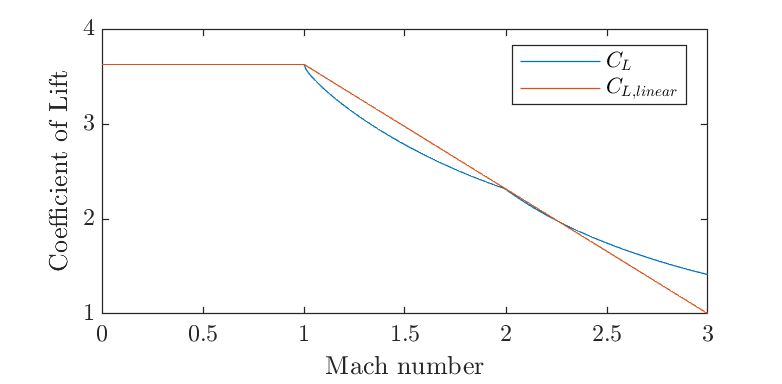
\includegraphics[width=0.5\linewidth]{images-design/airfoil_angles_linear.png}
    \caption[Canard airfoil approximation]{Canard airfoil approximation}
    \label{fig:jacobian-canard-airfoil}
\end{figure}

% which results in the Jacobians
% \begin{align}
%     C_{L \, v} &= 0 \quad\text{for}\quad \mathrm{Ma}\leq 1
%     \\
%     C_{L \, v} &= dt \, \alpha_c \frac{-4v c }{\sqrt{(v^2- c^2)^3}  }\quad\text{for}\quad \mu > \Lambda
%     \\
%     C_{L \, v} &=  dt \, \alpha_c
%     \frac{-0.3948 v \cot(\Lambda)^2 \left(129 c^2 \cot(\Lambda)^2 - 129 v^2 \cot(\Lambda)^2 + 19 c^2 + 226 c \cot(\Lambda) \sqrt{v^2 - c^2} \right)}
%     {c^3 \sqrt{v^2 - c^2} \left( \pi + \left(\cot(\Lambda) \sqrt{v^2 - c^2} \left(43 c^2 \cot(\Lambda)^2 - 43 v^2 \cot(\Lambda)^2 + 19 c^2 + 113 c \cot(\Lambda) \sqrt{v^2 - c^2} \right)\right)/(50 c^3) \right)^2 }
%     \quad\text{for}\quad \mu \leq \Lambda
%     \\
%     \implies
%     C_{L \, v} &\approx \bm 0
% \end{align}